\documentclass[12pt, a4paper]{article}
\usepackage{caption}
\usepackage{graphicx}
\usepackage{hyperref}
\hypersetup{
    colorlinks,
    citecolor=black,
    filecolor=black,
    linkcolor=black,
    urlcolor=black
}
\usepackage{tikz-network}
\usepackage{amsmath, amsfonts, amssymb, amsthm}
\usepackage{algpseudocode}
\usepackage{algorithm}
\title{Network and Cybersecurity\\ Assignment 2}
\date{2022}
\author{Kristoffer Klokker}

\usepackage{xcolor,listings}
\usepackage{textcomp}
\usepackage{color}
\usepackage{listings}
\definecolor{codegreen}{rgb}{0,0.6,0}
\definecolor{codegray}{rgb}{0.5,0.5,0.5}
\definecolor{codepurple}{HTML}{C42043}
\definecolor{backcolour}{HTML}{F2F2F2}
\definecolor{bookColor}{cmyk}{0,0,0,0.90}  
\color{bookColor}
\setcounter{tocdepth}{1}
\lstset{upquote=true}

\lstdefinestyle{mystyle}{
    backgroundcolor=\color{backcolour},   
    commentstyle=\color{codegreen},
    keywordstyle=\color{codepurple},
    numberstyle=\numberstyle,
    stringstyle=\color{codepurple},
    basicstyle=\footnotesize\ttfamily,
    breakatwhitespace=false,
    breaklines=true,
    captionpos=b,
    keepspaces=true,
    numbers=left,
    numbersep=10pt,
    showspaces=false,
    showstringspaces=false,
    showtabs=false,
    tabsize=3,
}
\lstset{style=mystyle}
\usepackage{zref-base}

\makeatletter
\newcounter{mylstlisting}
\newcounter{mylstlines}
\lst@AddToHook{PreSet}{%
  \stepcounter{mylstlisting}%
  \ifnum\mylstlines=1\relax
    \lstset{numbers=none}
  \else
    \lstset{numbers=left}
  \fi
  \setcounter{mylstlines}{0}%
}
\lst@AddToHook{EveryPar}{%
  \stepcounter{mylstlines}%
}
\lst@AddToHook{ExitVars}{%
  \begingroup
    \zref@wrapper@immediate{%
      \zref@setcurrent{default}{\the\value{mylstlines}}%
      \zref@labelbyprops{mylstlines\the\value{mylstlisting}}{default}%
    }%
  \endgroup
}

% \mylstlines print number of lines inside listing caption
\newcommand*{\mylstlines}{%
  \zref@extractdefault{mylstlines\the\value{mylstlisting}}{default}{0}%
}
\makeatother


\newcommand\numberstyle[1]{%
    \footnotesize
    \color{codegray}%
    \ttfamily
    \ifnum#1<10 0\fi#1 |%
}


\begin{document}
	\maketitle
	\clearpage
	\tableofcontents
	\clearpage
	\section{Problem - Congestion Control in TCP}
		\subsection{Describe TCP Cubic congestion control. Include a comparison to earlier versions (TCP Reno or TCP Tahoe), and explain why Cubic is chosen as the default in many operating systems today}
			TCP congestion controls a limit on the amount of traffic send by a TCP connection. This limit is known as the congestion window and is denoted $cwnd$.\\
			$cwnd$ is a variable used to getting the finding the limit of data through the network. The sending rate will roughly be equal to $\frac{cwnd}{RTT}bytes/sec$.
			To find the $cwnd$ value different approaches, TCP Reno, TCO Tahoe and Cubic all uses the first phase slow start.
			\subsubsection{Slow start}
				Slow start works by setting $cwnd=1$. When an acknowledgment then is gotten $cwnd$ is increased by 1 maximum segment size (MSS).\\
				This will therefore create an exponential growth.\\
				Once a loss is detected a new variable slow-start threshold $ssthresh$ is set equal to $cwnd/2$. Then $cwnd$ is set to 1 and slow start is repeated.\\
				In the event that $cwnd$ then get equal or higher than $ssthresh$ it will continue to next phase Congestion avoidance.\\
			\subsubsection{Congestion avoidance}
				Congestion avoidance works by using a different growing rate for $cwnd$ such the last maximum throughput $W_{max}$ will be hovered around.\\ 
				For TCP Tahoe and Reno the $cwnd$ is incremented every RTT.\\
				For TCP Cubic a variable $k$ is chosen which is the time which it should take a cubic function to reach the last known $W_{max}$.\\
				In case of a loss the $ssthresh$ value is set equal to half $cwnd$ and depending on type of congestion control different approaches is done.\\
				In case of a loss (triple duplicate ACKs or timeout) TCP Tahoe set $cwnd$ to 1 and goes to slow start.\\
				For TCP Reno and Cubic in case of timeout the $cwnd=cwnd/2$.\\
				In case of triple duplicate ACKs TCP Reno and Cubic goes to the Fast Recovery phase and set $cwnd=ssthresh+3MSS$\\
			\subsubsection{Fast recovery}
				For every duplicate ACKs that follows the $cwnd$ is increased by 1.\\
				This is done until the missing package ACK is received, an it returns to the Congestion avoidance phase.\\
				In case of a timeout $ssthresh$ is updated to half $cwnd$ and $cwnd$ is set to 1, from which Slow start is performed.
			\subsubsection{TCP Cubic's advantages}
				TCP Cubic has the same advantages over TCP Tahoe as TCP Reno.\\
				By not setting $cwnd$ to 1, a faster recovery is done in slow start. Moreover has the Fast recovery which helps not doing a complete reset in case of duplicate and faster recovers to the expected $W_{max}$.\\
				TCP Cubic has the advantage over TCP Reno by using a smart congestion avoidance function. By using a cubic function will it be assumed that limit for $W_{max}$ will be constant and therefore faster reach the constant and stay around it. In case of $W_{max}$ had gotten bigger, then the cubic function will grow faster than the linear functions and faster reach the new $W_{max}$.
	\section{Problem - RDI and Pipelining in TCP}
		The scenario is:
		\begin{itemize}
			\item There are 6 data segments (Numbered 1-6)
			\item The first time an ack if sent for segment 2, it is lost
			\item The first time segment 4 is sent, it is lost
			\item The window size is fixed at 3
		\end{itemize}
		\subsection{Draw a timing diagram for RDT pipelining in TCP given the scenario described above. Make sure your diagram show when data is delivered to the application layer. Include a description where you point out the TCP specific elements.}
		\begin{figure}[h]
			\centering
			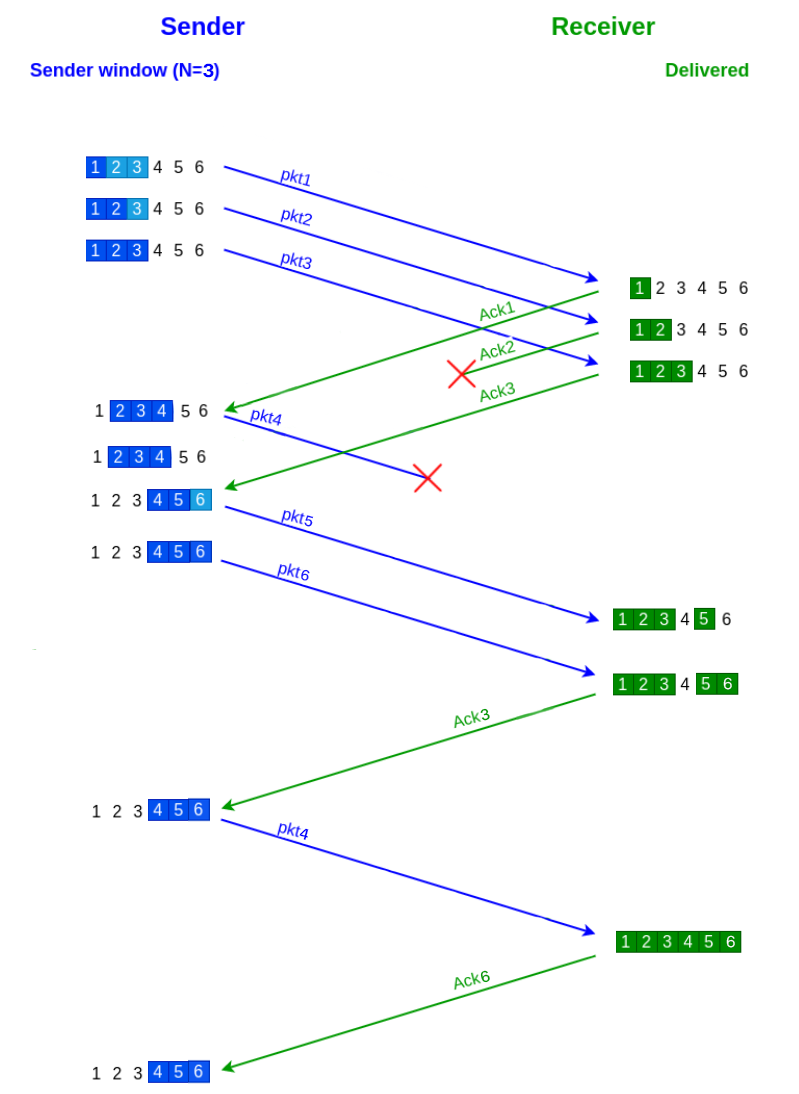
\includegraphics[width=250px]{assets/RDT.png}
			\caption{RDT pipelining in TCP}
			\label{fig:RDT}
		\end{figure}
		In the diagram \ref{fig:RDT} is buffer colors representing:
		\begin{itemize}
			\item Darkblue is the sent segments
			\item Lightblue is the segments in the sending window 
			\item Dark green are the received segments which is in the receiver buffer ready for the application layer to stream.
		\end{itemize}
		When the acknowledgement 2 is lost, will commutative acknowledgement tell the sender that segment 2 was received, due to receiving acknowledgement 3.\\
		When the segment 4 is lost is assumed that the receiver will buffer segment 5 and 6, from this it can be seen that segment 3 is acknowledged again indicating that segment 4 was lost. When segment 4 is then received the buffered segments are still used such the last segment 6 is acknowledged. This is again using commutative acknowledgement.
	\section{Problem - TLS}
		Consider the picture in figure \ref{fig:wireshark} of a package captured form wireshark. Answer the questions below the image.
		\begin{figure}[h]
			\centering
			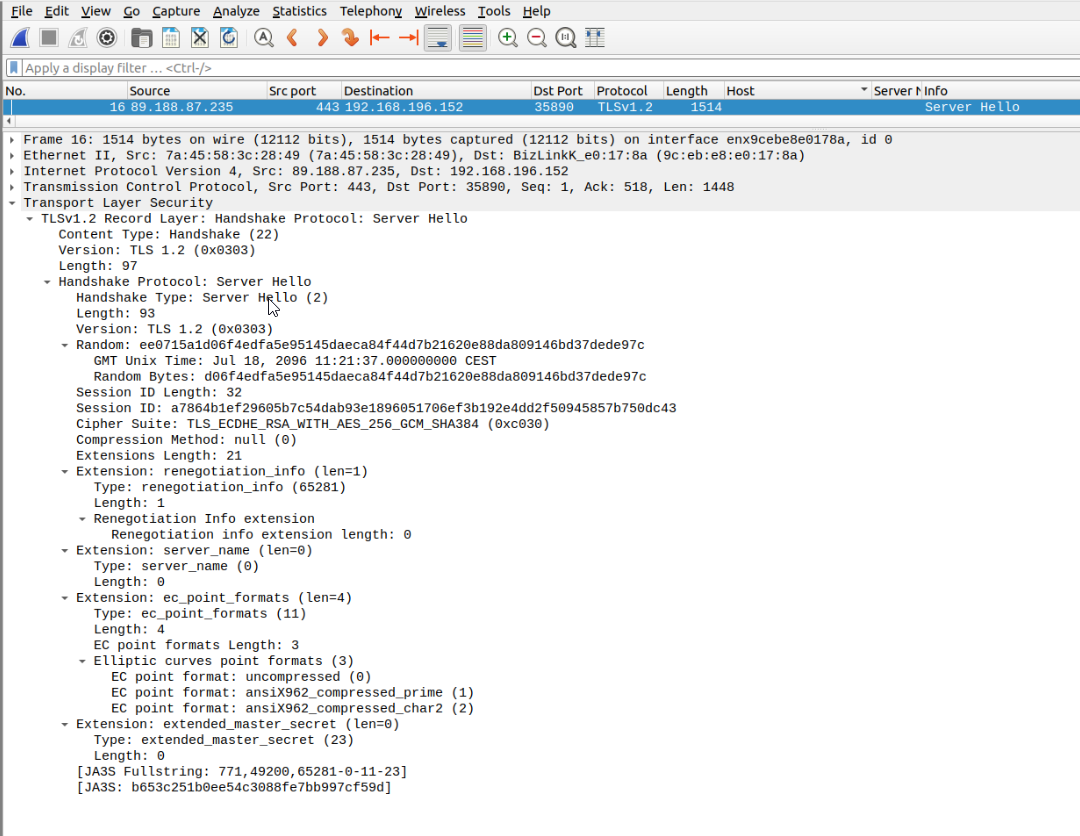
\includegraphics[width=300px]{assets/wireshark.png}
			\caption{Wireshark capture}
			\label{fig:wireshark}
		\end{figure}
		\subsection{What is the overall role of the highlighted packet (packet No 16)?}
			The packets role is the answer to a client hello.\\
			The server hello package contain:
			\begin{itemize}
				\item Choice of cryptography,- and hashing algorithms
				\item SSL certificate
				\item Random string of bytes (nonce)
			\end{itemize}
		\subsection{What was the length of the data in the previous packet?}
			While starting the connection and sending the SYN flag, the ack number will be 1.\\
			It can be seen that the current ACK number is 518, therefore making the last package sent of size 517 bytes.
		\subsection{What version of TLS is being used, and which cipher suite is used?}
			The TLS version used is 1.2\\
			The ciphers used are:
			\begin{itemize}
				\item Key Exchange -  ECDHE (Elliptic Curve Diffie-Hellman Ephemeral)
				\item Authentication - RSA (Rivest Shamir Adleman)
				\item Encryption - AES (Advanced Encryption Standard) 256 with Galois/Counter mode
				\item Hash - SHA (Secure Hash Algorithm) 384
			\end{itemize}
		\subsection{Who selected the cipher suite, the client of the server?}
			In TLS the server always selects cipher suite, which it desires from the offered ones by the client.
		\subsection{What does each parts of the cipher suite provide to TLS?}
			\begin{itemize}
				\item Key Exchange - The keys used for encryption and decryption of package data
				\item Authentication - The authentication algorithm is used to ensure authentication between client and server
				\item Encryption - The chosen algorithm for encrypting and decrypting the package data to ensure confidentiality
				\item Hash - The hashing method for ensuring integrity of the data
			\end{itemize}
			
\end{document}
